\documentclass[a4paper,12pt]{report}

\usepackage[utf8x]{inputenc}
\usepackage[T2A]{fontenc}
\usepackage[english, russian]{babel}

% Опционно, требует  apt-get install scalable-cyrfonts.*
% и удаления одной строчки в cyrtimes.sty
% Сточку не удалять!
% \usepackage{cyrtimes}

% Картнки и tikz
\usepackage{graphicx}
\usepackage{tikz}
\usetikzlibrary{snakes,arrows,shapes}


% Увы, поля придётся уменьшить из-за листингов.
\topmargin -1cm
\oddsidemargin -0.5cm
\evensidemargin -0.5cm
\textwidth 17cm
\textheight 24cm

\sloppy



% Оглавление в PDF
\usepackage[
bookmarks=true,
colorlinks=true, linkcolor=black, anchorcolor=black, citecolor=black, menucolor=black,filecolor=black, urlcolor=black,
unicode=true
]{hyperref}

% Для исходного кода в тексте
% \newcommand{\Code}[1]{\texttt{#1}}

% Некоторая русификация.
% \usepackage{misccorr} % Oh shi^W^W, оно не работает с report.
\usepackage{indentfirst}
\renewcommand{\labelitemi}{\normalfont\bfseries{--}}

% На дворе XXI век, но пакет listings всё ещё не пашет с русскими комментариями!

% Пакет listings для простой вставки исходников
% \usepackage{listings}
% Параметры оформления
% \lstset{
% showspaces=false,
% showtabs=false,
% frame=single,
% tabsize=4,
% basicstyle=\ttfamily,
% identifierstyle=\ttfamily,
% commentstyle=\itshape,
% stringstyle=\ttfamily,
% keywordstyle=\ttfamily,
% breaklines=true
% }
% Русский в комментариях.
% \lstset{escapebegin=\begin{cyr},escapeend=\end{cyr}}



% А это взято из файла, сгенерённого doxygen
\usepackage{calc}
\usepackage{array}
\newenvironment{Code}
{\footnotesize}
{\normalsize}
\newcommand{\doxyref}[3]{\textbf{#1} (\textnormal{#2}\,\pageref{#3})}
\newenvironment{DocInclude}
{\footnotesize}
{\normalsize}
\newenvironment{VerbInclude}
{\footnotesize}
{\normalsize}
\newenvironment{Image}
{\begin{figure}[H]}
{\end{figure}}
\newenvironment{ImageNoCaption}{}{}
\newenvironment{CompactList}
{\begin{list}{}{
  \setlength{\leftmargin}{0.5cm}
  \setlength{\itemsep}{0pt}
  \setlength{\parsep}{0pt}
  \setlength{\topsep}{0pt}
  \renewcommand{\makelabel}{\hfill}}}
{\end{list}}
\newenvironment{CompactItemize}
{
  \begin{itemize}
  \setlength{\itemsep}{-3pt}
  \setlength{\parsep}{0pt}
  \setlength{\topsep}{0pt}
  \setlength{\partopsep}{0pt}
}
{\end{itemize}}
\newcommand{\PBS}[1]{\let\temp=\\#1\let\\=\temp}
\newlength{\tmplength}
\newenvironment{TabularC}[1]
{
\setlength{\tmplength}
     {\linewidth/(#1)-\tabcolsep*2-\arrayrulewidth*(#1+1)/(#1)}
      \par\begin{tabular*}{\linewidth}
             {*{#1}{|>{\PBS\raggedright\hspace{0pt}}p{\the\tmplength}}|}
}
{\end{tabular*}\par}
\newcommand{\entrylabel}[1]{
   {\parbox[b]{\labelwidth-4pt}{\makebox[0pt][l]{\textbf{#1}}\vspace{1.5\baselineskip}}}}
\newenvironment{Desc}
{\begin{list}{}
  {
    \settowidth{\labelwidth}{40pt}
    \setlength{\leftmargin}{\labelwidth}
    \setlength{\parsep}{0pt}
    \setlength{\itemsep}{-4pt}
    \renewcommand{\makelabel}{\entrylabel}
  }
}
{\end{list}}
\newenvironment{Indent}
  {\begin{list}{}{\setlength{\leftmargin}{0.5cm}}
      \item[]\ignorespaces}
  {\unskip\end{list}}


\begin{document}

\maketitle

\tableofcontents

\addcontentsline{toc}{chapter}{Введение}
\chapter*{Введение}
\subsection{Цели и задачи}

Цель: 
    Разработать \textbf{SMTP-сервер} с использованием рабочих процессов и select.

Задачи:
\begin{itemize}
    \item Проанализировать архитектурное решение
    \item Разработать подход для обработки входящих соединений и хранения входящих писем в maildir
    \item Рассмотреть \textbf{SMTP}-протокол
    \item Реализовать программу для получения писем по протоколу \textbf{SMTP}
\end{itemize}

\chapter{Аналитический раздел}

\section*{Предметная область}
\subsection*{ER-диаграмма предметной области}
Согласно обозначенному протоколу в рамках данной работы, в системе устанавливаются отношения "отправитель - получатель", причем отправитель может отправить несколько писем, указав себя в качестве источника сообщения (единственного). Основная единица данных, передаваемая по протоколу - письмо, которое включает в себя отправителя и получателя, причем получателей может быть несколько. Также письмо содержит в себе единственное тело, которое может быть использовано как для последующей передачи, так и для хранения на сервере.
Таким образом, в рамках предметной области можно выделить 4 вида сущностей:
\begin{itemize}
    \item 1. Отправитель
    \item 2. Получатель
    \item 3. Письмо
    \item 4. Тело письма
\end{itemize}
Зависимость между сущностями предметной области может быть описана следующей диаграммой (~\ref{fig:er_diagram} ):
\begin{figure}
\centering
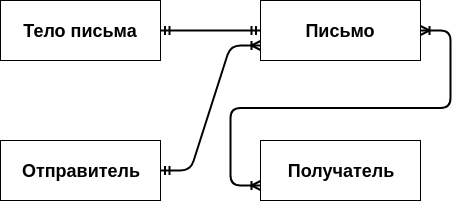
\includegraphics[width=\textwidth]{static/ER_diagram_field.png}
\caption{ER-диаграмма сущностей}
\label{fig:er_diagram}
\end{figure}

\section*{Сервер}
\subsection*{Преимущества и недостатки условия задачи}
Согласно условию задачи, в работе сервера предлагается исполльзовать многопроцессную систему. Данный тип системы
является самым простым в плане разработки при условии, что на каждую пользовательскую сессию или даже любой пользовательский запрос
создается новый процесс. Данная архитектура имеет следующие преимущества:
\begin{itemize}
    \item 1. Простота разработки. Фактически, мы запускаем много копий однопоточного приложения и они работают независимо друг от друга. Можно не использовать никаких специфически многопоточных API и средств межпроцессного взаимодействия.
    \item 2. Высокая надежность. Аварийное завершение любого из процессов никак не затрагивает остальные процессы.
    \item 3. Хорошая переносимость. Приложение будет работать налюбой многозадачной ОС
    \item 4. Высокая безопасность. Разные процессы приложения могут запускаться от имени разных пользователей. Таким образом можно реализовать принцип минимальных привилегий, когда каждый из процессов имеет лишь те права, которые необходимы ему для работы. Даже если в каком-то из процессов будет обнаружена ошибка, допускающая удаленное исполнение кода, взломщик сможет получить лишь уровень доступа, с которым исполнялся этот процесс.
\end{itemize}
При этом данная архитектура имеет следующие недостатки:
\begin{itemize}
    \item 1. Далеко не все прикладные задачи можно предоставлять таким образом. Например, эта архитектура годится для сервера, занимающегося раздачей статических HTMLстраниц, но совсем непригодна для сервера баз данных и многих серверов приложений.
    \item 2. Создание и уничтожение процессов – дорогая операция, поэтому для многих задач такая архитектура неоптимальна.
\end{itemize}
Поэтому для минимизации операций создания и уничтожения процессов предлагается архитектурное решение, представляющее собой пул процессов,
создаанных заранее. Это позволит фиксировать число операций создания процесса. При этом слушающие сокеты сервера должны наследоваться каждым создаваемым процессом. Это делается для решения проблемы распределения соединений между процессами одной группы. В ходе исследования предметной области и реализации сервера с заданной архитектурой, было выяснено, что открытые файловые дескрипторы процесса не могут быть переданы посредством очередей сообщений. (при передаче открытого дескриптора возникает ошибка EBADF). Однако система с наследованием имеет недостаток в отсутствии возможности распределения соединений между процессами - соединение принимает тот, кто быстрее успел.

\chapter{Конструкторский раздел}

\section{Конечный автомат состояний сервера}

Конечный автомат состояний сервера представлен на Рис.~\ref{fig:server_fsm} 

\begin{figure}
\centering
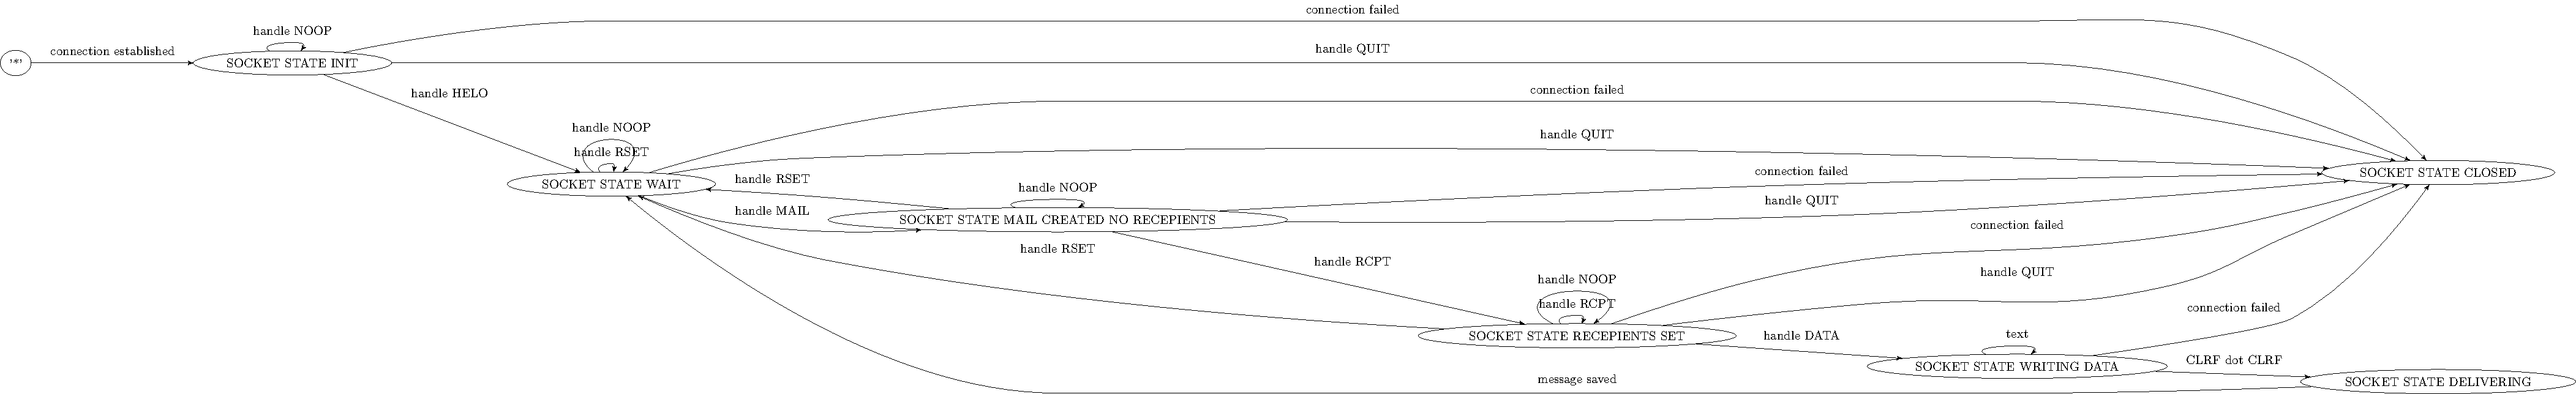
\includegraphics[width=\textwidth]{static/server_dot.pdf}
\caption{Состояния сервера}
\label{fig:server_fsm}
\end{figure}

\subsection{Синтаксис команд протокола}
Ниже приведен формат команд сообщений протокола в виде регулярных выражений
\begin{enumerate}
\item \textbf{EHLO}: {\it EHLO [w+]+\/}
\item \textbf{HELO}: {\it HЕLO [w+]+\/}
\item \textbf{MAIL}: {\it MAIL FROM <[\textbackslash w]+@[\textbackslash w]+\.[\textbackslash w]+>\/}
\item \textbf{RCPT}: {\it RCPT <[\textbackslash w]+@[\textbackslash w]+\.[\textbackslash w]+>\/}
\item \textbf{DATA}: {\it DATA\/}
\item \textbf{VRFY}: {\it VRFY [w+]+\/}
\item \textbf{RSET}: {\it RSET\/}
\item \textbf{QUIT}: {\it QUIT\/}
\end{enumerate}

\subsection*{Представление данных}
Ниже приведены диаграммы представления данных в системе - логическая и физическая.

\begin{figure}
\centering
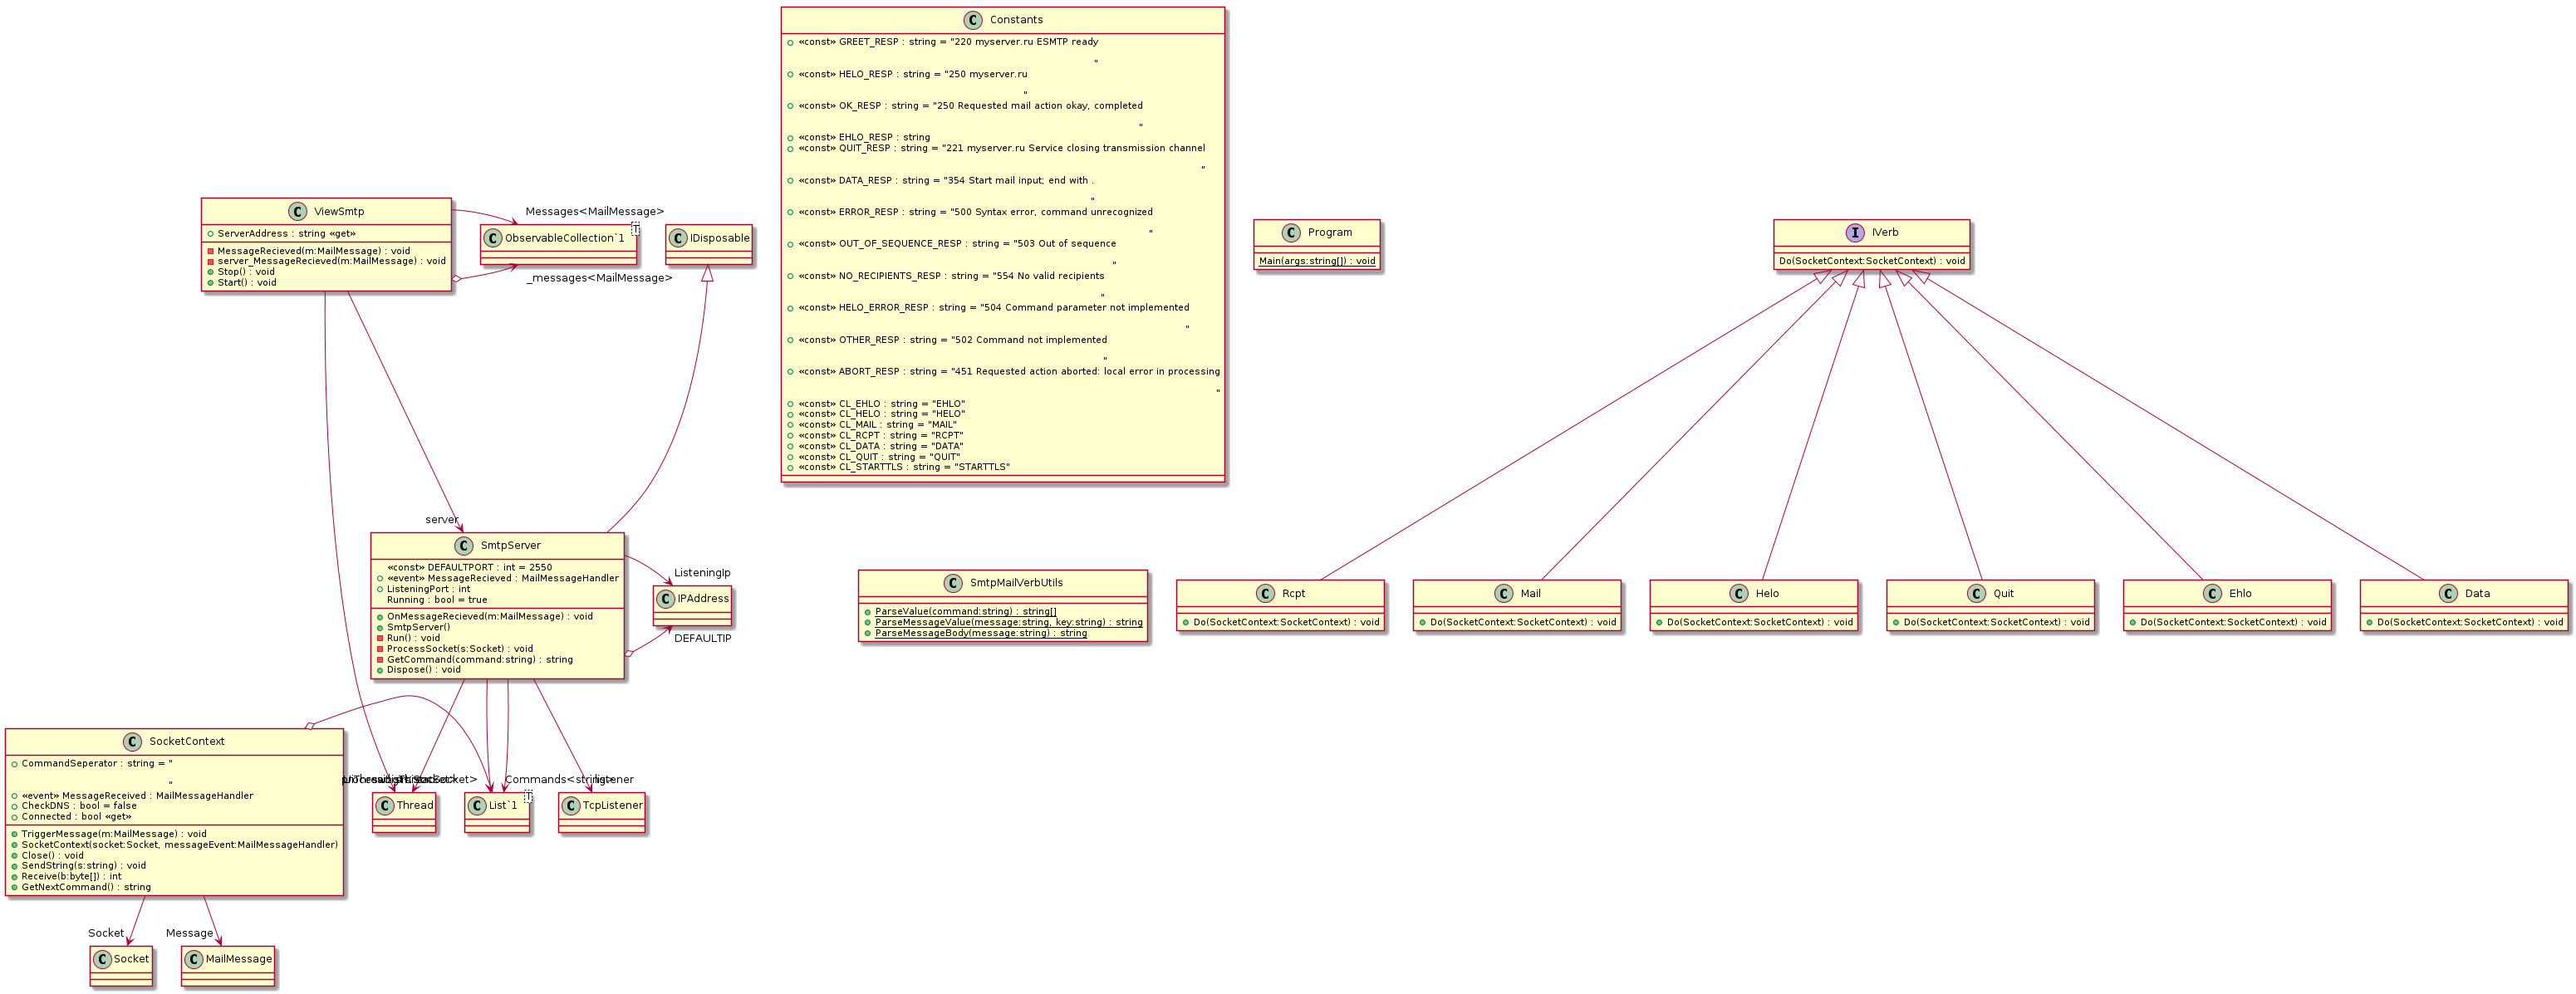
\includegraphics[width=\textwidth]{static/Server_Class_Diagram.png}
\caption{Логическая диаграмма сущностей}
\label{fig:logic_diagram}
\end{figure}

\begin{figure}
\centering
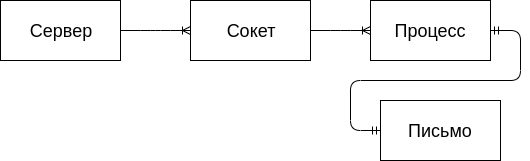
\includegraphics[width=\textwidth]{static/physical.png}
\caption{Физическая диаграмма сущностей}
\label{fig:phys_diagram}
\end{figure}

\subsection{Алгоритм обработки соединений}
\begin{verbatim}


 ПОКА (процесс_работает == 1) 
      Добавить дескрипторы слушающих сокетов в сет читателей 
      Добавить дескрипторы клиентских сокетов в сет читателей 
      Ожидать соединения на одном из сокетов (время = 5с) 
      ЕСЛИ есть запрос ТО 
        ДЛЯ каждого слушающего сокета 
           ЕСЛИ действие на одном из слушающих сокетов ТО 
               Принять новое соединение 
               Инициализировать новый сокет 
               Отправить приветствие 
               Установить неблокирующий режим для принятого соединения 
           КОНЕЦ ЕСЛИ 
        КОНЕЦ ДЛЯ 
        ДЛЯ каждого клиентского сокета 
           ЕСЛИ действие на одном из клиентских сокетов ТО 
              Обработать действие в соответствии с протоколом 
           КОНЕЦ ЕСЛИ 
        КОНЕЦ ДЛЯ 
      КОНЕЦ ЕСЛИ 
 КОНЕЦ ПОКА 

\end{verbatim}

\chapter{Технологический раздел}

\section{Сборка программы}

Сборка программы описана в файле \textit{Makefile} системы сборки \textit{make}. Рис.~\ref{fig:make} нагенерили \textit{makefile2dot}.

\begin{figure}
\centering
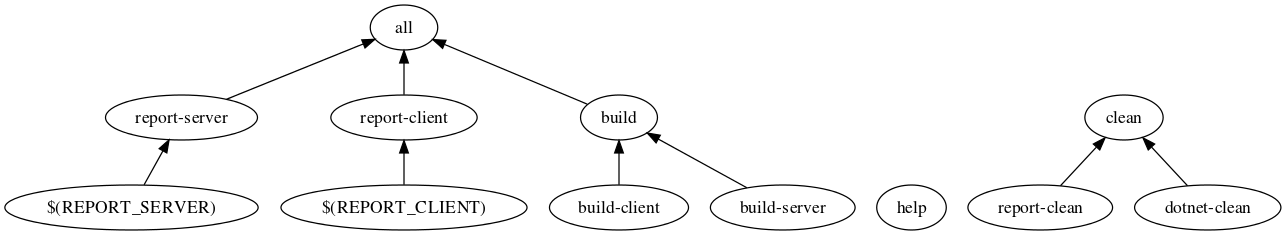
\includegraphics[width=\textwidth]{include/make.png}
\caption{Сборка программы}
\label{fig:make}
\end{figure}

\section{Графы вызова функций}

Поскольку функций много, графы вызовов разбиты на два рисунка. На рис.~\ref{fig:cflow01} показаны основные функции, на рис.~\ref{fig:cflow02}~-- функции обработки команд. 

\begin{figure}
\centering
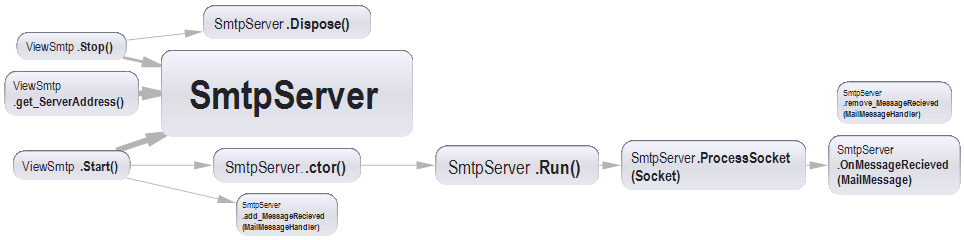
\includegraphics[width=\textwidth]{include/cflow1.png}
\caption{Граф вызовов, основные функции}
\label{fig:cflow01}
\end{figure}

\begin{figure}
\centering
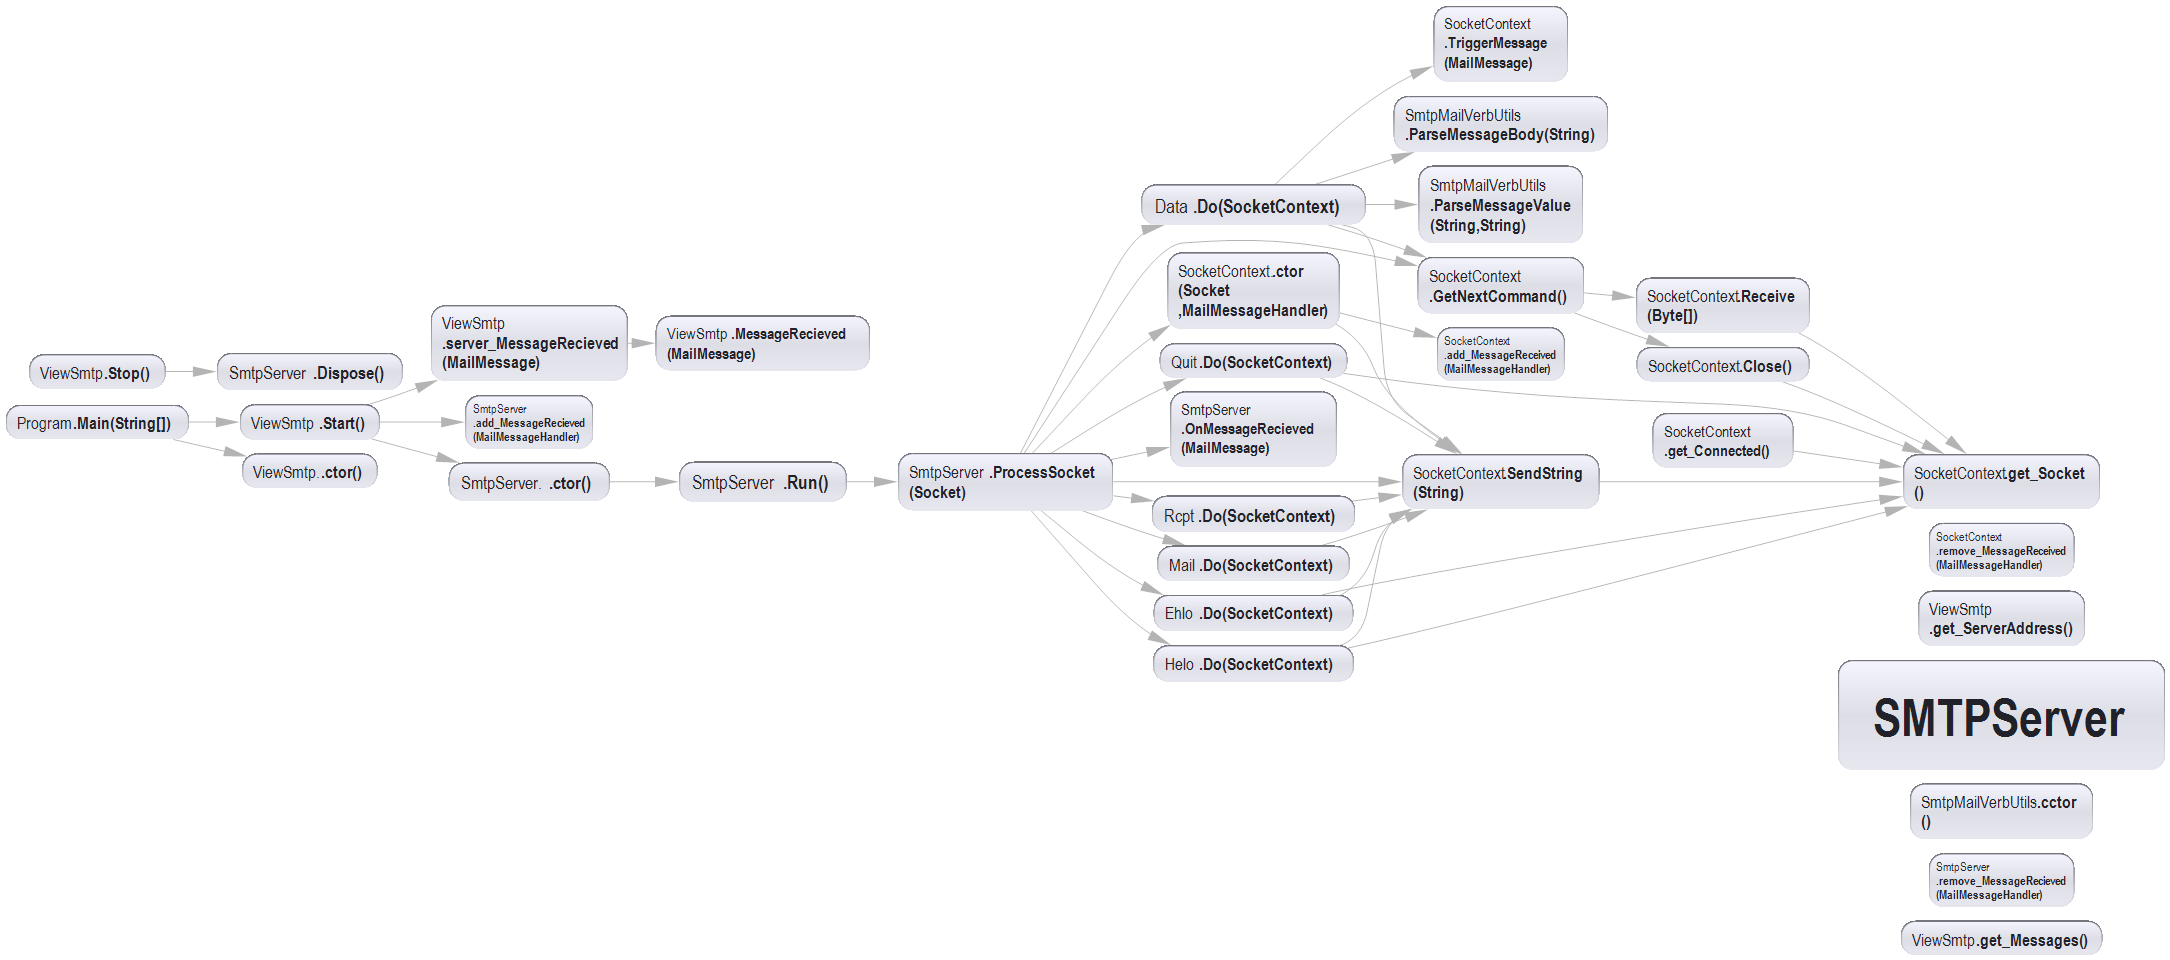
\includegraphics[width=\textwidth]{include/cflow2.png}
\caption{Граф вызовов, функции обработки команд}
\label{fig:cflow02}
\end{figure}

Графы созданы с помощью \textit{nDepend}.

\vspace{100mm}

\section{Тестирование}

Ниже приведён отчет о модульном тестировании.

\begin{verbatim}

Server: 504 Command parameter not implemented
HELO Test: success
Server: 504 Command parameter not implemented
EHLO Test: success
Server: 250 Requested mail action okay, completed
MAIL Test1: success
Server: 500 Syntax error, command unrecognized
MAIL Test2: success
Server: 500 Syntax error, command unrecognized
RCPT Test1: success
Server: 250 Requested mail action okay, completed
RCPT Test2: success
Server: 250 Requested mail action okay, completed
RCPT Test3: success
Server: 252 Cannot VRFY user, but will accept message and attempt delivery
VRFY Test: success
Server: 503 Out of sequence
DATA Test1: success
Server: 554 No valid recipients
DATA Test2: success
Server: 354 Start mail input; end with .
250 Requested mail action okay, completed
DATA Test3: success
Server: 354 Start mail input; end with .
500 Syntax error, command unrecognized
DATA Test4: success
Server: 250 Requested mail action okay, completed
RSET Test1: success
Server: 250 Requested mail action okay, completed
RSET Test2: success
Server: 221 myserver.ru Service closing transmission channel
QUIT Test: success

RunTime 00:00:00.14

\end{verbatim}
\addcontentsline{toc}{chapter}{Выводы}
\chapter*{Выводы}

В рамках предложенной работы нами были реализованы два компонента современного SMTP-сервера, взаимодействующих между самой по самописному протоколу в соответствии со стандартами RFC. В ходе работы реализованы следующие задачи: \\
\begin{enumerate}
	\item Проанализировали архитектурное решение
    \item Разработали подход для обработки входящих соединений и хранения входящих писем в maildir
    \item Рассмотрели \textbf{SMTP}-протокол
    \item Реализовали программу для получения писем по протоколу \textbf{SMTP}
    \item Рассмотрели работу с неблокирующими сокетами и их взаимодействие 
    \item Разработали системы, работающие в многозадачном режиме, столкнувшись с проблемами взаимодействия процессов, которые были решены в ходе работы
    \item Познакомились с утилитами автоматической сборки и тестирования
\end{enumerate}


\end{document}
